% !TEX TS-program = xelatex
% !TEX encoding = UTF-8 Unicode 

% \documentclass[AutoFakeBold]{LZUThesis}
\documentclass[AutoFakeBold]{LZUThesis}
\usepackage{multirow}
\usepackage{threeparttable}
\usepackage{booktabs} % 导入三线表需要的宏包
\usepackage{longtable}% 导入跨页表格所需宏包


\CTEXsetup[name={第,部分}]{chapter}
\lstset{
language = MATLAB,
backgroundcolor=\color{white},   % choose the background color; you must add \usepackage{color} or \usepackage{xcolor}  
basicstyle=\footnotesize,        % the size of the fonts that are used for the code  
breakatwhitespace=false,         % sets if automatic breaks should only happen at whitespace  
breaklines=true,                 % sets automatic line breaking  
captionpos=bl,                    % sets the caption-position to bottom  
% commentstyle=\color{green},    % comment style  
% deletekeywords={...},            % if you want to delete keywords from the given language  
% escapeinside={\%*}{*)},          % if you want to add LaTeX within your code  
extendedchars=true,              % lets you use non-ASCII characters; for 8-bits encodings only, does not work with UTF-8  
frame=shadowbox,                    % adds a frame around the code  
keepspaces=true,                 % keeps spaces in text, useful for keeping indentation of code (possibly needs columns=flexible)  
keywordstyle=\color{blue},       % keyword style  
% language=Python,                 % the language of the code  
morekeywords={*,...},            % if you want to add more keywords to the set  
numbers=left,                    % where to put the line-numbers; possible values are (none, left, right)  
numbersep=5pt,                   % how far the line-numbers are from the code  
numberstyle=\tiny\color{gray}, % the style that is used for the line-numbers  
rulecolor=\color{black},         % if not set, the frame-color may be changed on line-breaks within not-black text (e.g. comments (green here))  
showspaces=false,                % show spaces everywhere adding particular underscores; it overrides 'showstringspaces'  
showstringspaces=false,          % underline spaces within strings only  
showtabs=false,                  % show tabs within strings adding particular underscores  
stepnumber=1,                    % the step between two line-numbers. If it's 1, each line will be numbered  
stringstyle=\color{orange},     % string literal style  
tabsize=2,                       % sets default tabsize to 2 spaces  
% title=signalAnalysis.m           % show the filename of files included with \lstinputlisting; also try caption instead of title  
}  

\begin{document}
%=====%
%
%封皮页填写内容
%
%=====%

% 标题样式 使用 \title{{}}; 使用时必须保证至少两个外侧括号
%  如: 短标题 \title{{第一行}},  
% 	      长标题 \title{{第一行}{第二行}}
%             超长标题\tiitle{{第一行}{...}{第N行}}

\title{{基于Nios ii 软核的频率计实现}}



% 标题样式 使用 \entitle{{}}; 使用时必须保证至少两个外侧括号
%  如: 短标题 \entitle{{First row}},  
% 	      长标题 \entitle{{First row}{ Second row}}
%             超长标题\entitle{{First row}{...}{ Next N row}}
% 注意:  英文标题多行时 需要在开头加个空格 防止摘要标题处英语单词粘连.

\author{\CJKfontspec{楷体}李文涛}
\major{电子信息基地班}
\college{320200928101}
\grade{2020级}



\maketitle
\frontmatter

% %中文摘要
% \ZhAbstract{
%     本文主要介绍了对电子交通灯的功能需求进行分析的过程,将其功能拆分,利用模块化设计的思想
%     将功能一步步实现,完成时钟信号产生模块、倒计时模块、红绿灯显示模块、倒计时数字化显示模块,
%     然后将各功能模块组合在一起实验完整的电子交通灯系统。
%     通过完整地进行对电子信号灯的设计,了解了电子设计的基本过程,具备初步独立设计电子系统的能力,
%     认识到模块化设计和提前整体设计布局的重要性。
% }
% {电子交通灯,模块化设计,整体设计布局}


% %英文摘要
% \EnAbstract{This paper mainly introduces the process of analyzing the functional requirements of the electronic traffic light, splitting its functions and using the idea of modular design
% The functions will be realized step by step, complete the clock signal generation module, countdown module, traffic light display module, countdown digital display module,
% Then the functional modules are combined together to experiment the complete electronic traffic light system.
% Through the complete design of the electronic signal lamp, I understand the basic process of electronic design, and have the ability to design the electronic system independently.
% Recognize the importance of modular design and overall layout in advance.
%     \fontspec{Times New Roman}}
% {Electronic traffic lights, modular design, overall design layout}

% %生成目录
% % \tableofcontents
% % \addcontentsline{toc}{chapter}{目录}
% % \thispagestyle{empty}


%文章主体
\mainmatter

\chapter{实验依赖}

\section{实验目的}
本次实验项目使用Quartus II、SOPC Builder(Qsys)、Nios II等从零开始构建一个能够在DE2-70实验平台上运行的uC/OS-II操作系统的Nios II系统,并在此基础上实现同时适用于高频和低频的频率计。由于DE2-70实验平台实验平台有困难,后使用野火的EP4CE10F17C8开发板实现。

\section{实验环境}
Quartus II 13.0 + 野火征途 Altera EP4CE10F17C8

(1)Quartus II 13.0:此版本的Quartus II较新,没有内置库,需要提前自行下载。对于野火的EP4CE10F17C8,下载Cyclone IV E库即可;对于DE2-70,需要下载Cyclone II库,由于太古老,安装库失败,建议使用Quartus II 9.0(已内置库),但使用过程中出现问题较多

(2)野火征途 Altera EP4CE10F17C8:简单介绍此次开发板上我们需要用到的部分板块。

A. EP4CE10主芯片:该芯片为开发板的主芯片,即FPGA芯片,其型号为 EP4CE10F17C8。该芯片拥有10k的逻辑单元,179个可配置的I/O口,414kbit的嵌入式RAM资源(每9kbit容量为一个块,每块为一个嵌入式存储单元,即有46个嵌入式存储单元),两个独立PLL锁相环,10个全局时钟网络。

B. SDRAM:板载 SDRAM 芯片,SDRAM 是一个同步动态随机存储器。这里我们使用的 SDRAM 芯片型号为 W9825G6KH-6,容量为 256Mbit。在设计时不能超过其最大容量。

C. 下载接口(JTAG):FPGA下载器通过该接口与开发板连接,用于程序的下载、固化以及调试。

D. 数码管:征途Pro开发板上配置了六位八段数码管,同时搭载了两块 74HC595 芯片,74HC595具有串行输入,并行输出的功能。使用该芯片的四位控制信号即可输出14位的数码管控制信号,这样可以大大地节省IO口资源。

E. LED显示灯:板载四个 led 显示灯(蓝灯),这四个 led 灯可以作为程序的状态显示灯。可以设计通 过 led 灯来判断程序是否正确执行,在调试时可以起到辅助作用。
\section{实验原理}
本次设计实现的前提是构建Nios II系统作为一个简单的单片机结构,并在此基础上增添频率计。

Nios II是Altera(2015年被Intel收购)为其FPGA所设计的一种RSIC架构的嵌入式软核处理器。

RSIC:精简指令集。

软核处理器:使用FPGA的硬件资源搭建起来的处理器。

硬件处理器:芯片内集成的硬件电路所形成的处理器。

为了使频率计既可以测定高频又可以测定低频,本次频率计中一共使用了两种不同的测定方法:

(1)频率测量法(计频法):单位时间内,信号周期变化的次数。假设时间为T,那么我们在T时间内周期数为N,那么我们就可以计算出频率,即f=N/T。此种方法适用于高频信号的测量,并且会出现±1的误差,对于低频误差会更大。

(2)周期测量法(计时法):先测量被测信号的时钟周期T,然后根据f=1/T,求出被测时钟的频率,先测量第一个上升沿的时间,然后测量第二个上升沿的时间,两个相减,就是时钟周期T,然后取倒数就是时钟频率。当频率比较低时,测量两个上升沿的时间是比较容易的,但是频率较高时,就比较难满足要求。因此这种方法适用于低频信号的测量。

\chapter{实验步骤}
\section{新建工程}
File→New Project Wizard,填写好工程的路径和名称点击Finish,选好芯片,完成工程的创建。芯片型号选择如下图
\begin{figure}[htbp]
    \centering
    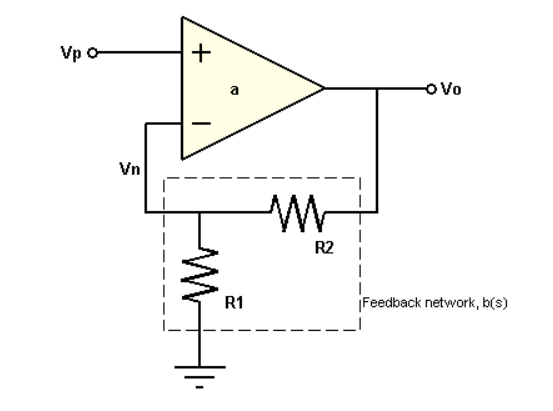
\includegraphics[width=350pt]{1.png}
\end{figure}
\section{搭建SOPC系统}
A. Tools→Qsys

B. 保存文件:File→Save

C. 设置系统时钟频率为50MHz

\begin{figure}[htbp]
    \centering
    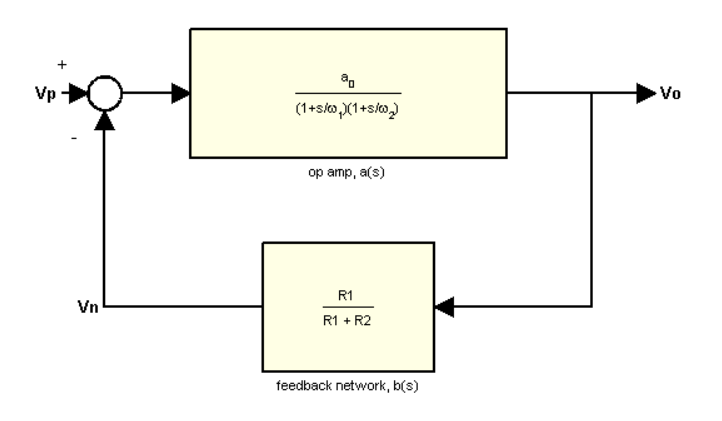
\includegraphics[width=350pt]{2.png}
    \caption{C. 设置系统时钟频率为50MHz}
\end{figure}

D. 添加Nios II Processor、jtag、sdram、PLL等等,并将IP核连接起来(连接时钟信号、复位信号、数据总线、取指令端口、复位端口、中断信号),并更改对应的名字;添加片System ID Peripheral核,保持默认选项即可。

\begin{figure}[htbp]
    \centering
    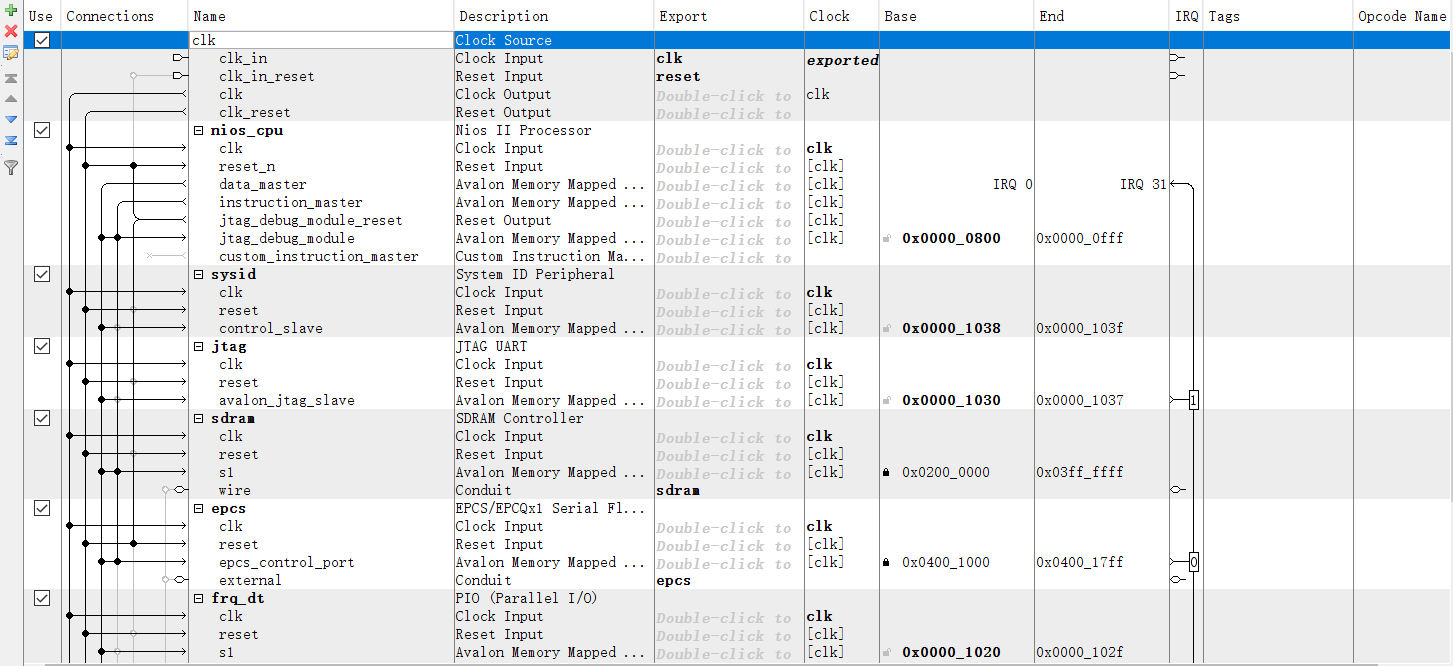
\includegraphics[width=350pt]{3.png}
    \caption{D. 添加Nios II Processor、jtag、sdram、PLL}
\end{figure}

E. 添加PIO接口,分别命名为frq\_dt、frq\_cs、ext\_int。

\begin{figure}[htbp]
    \centering
    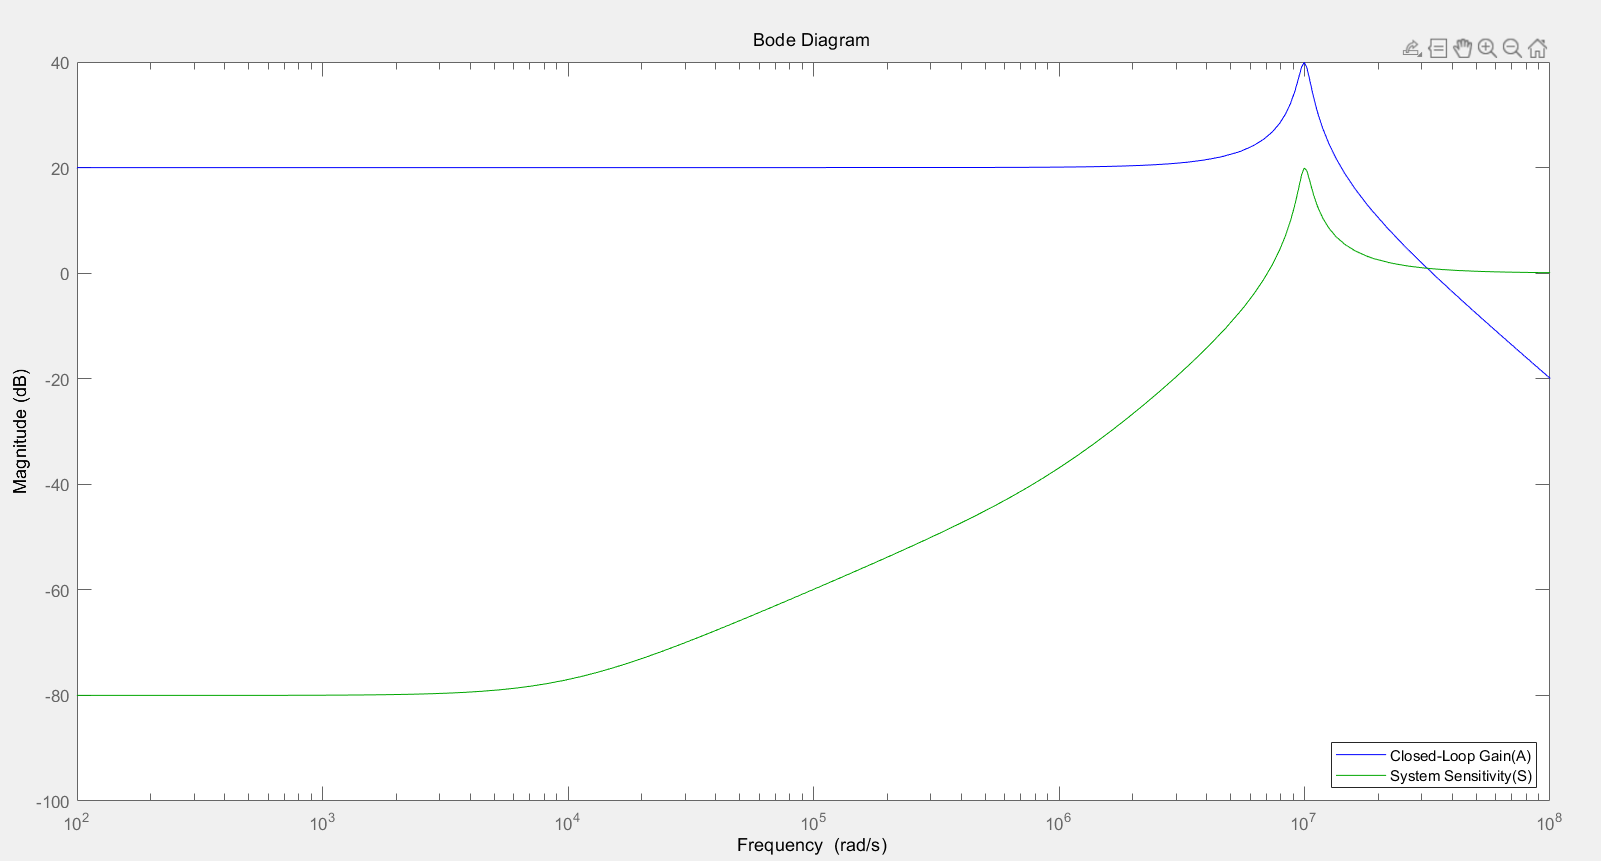
\includegraphics[width=350pt]{4.png}
    \caption{E. 添加PIO接口,分别命名为frq\_dt、frq\_cs、ext\_int}
\end{figure}

F. 进行地址分配,点击Qsys主界面菜单栏中的“system”下的“Assign Base Address”。

\begin{figure}[htbp]
    \centering
    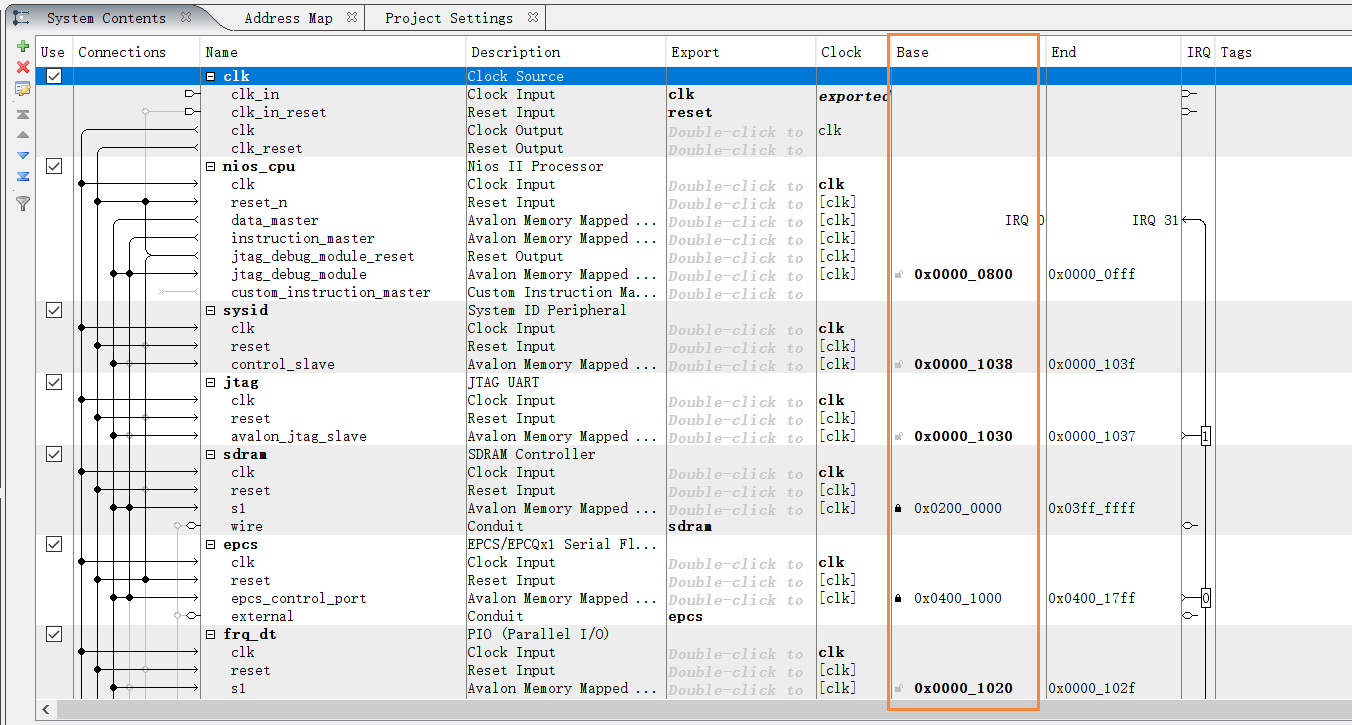
\includegraphics[width=350pt]{5.png}
    \caption{F. 进行地址分配}
\end{figure}

G. 分配中断号,在“IRQ”标签栏下点选“Avalon\_xxx”和IRQ的连接点就会给对应设备添加中段号。

\begin{figure}[htbp]
    \centering
    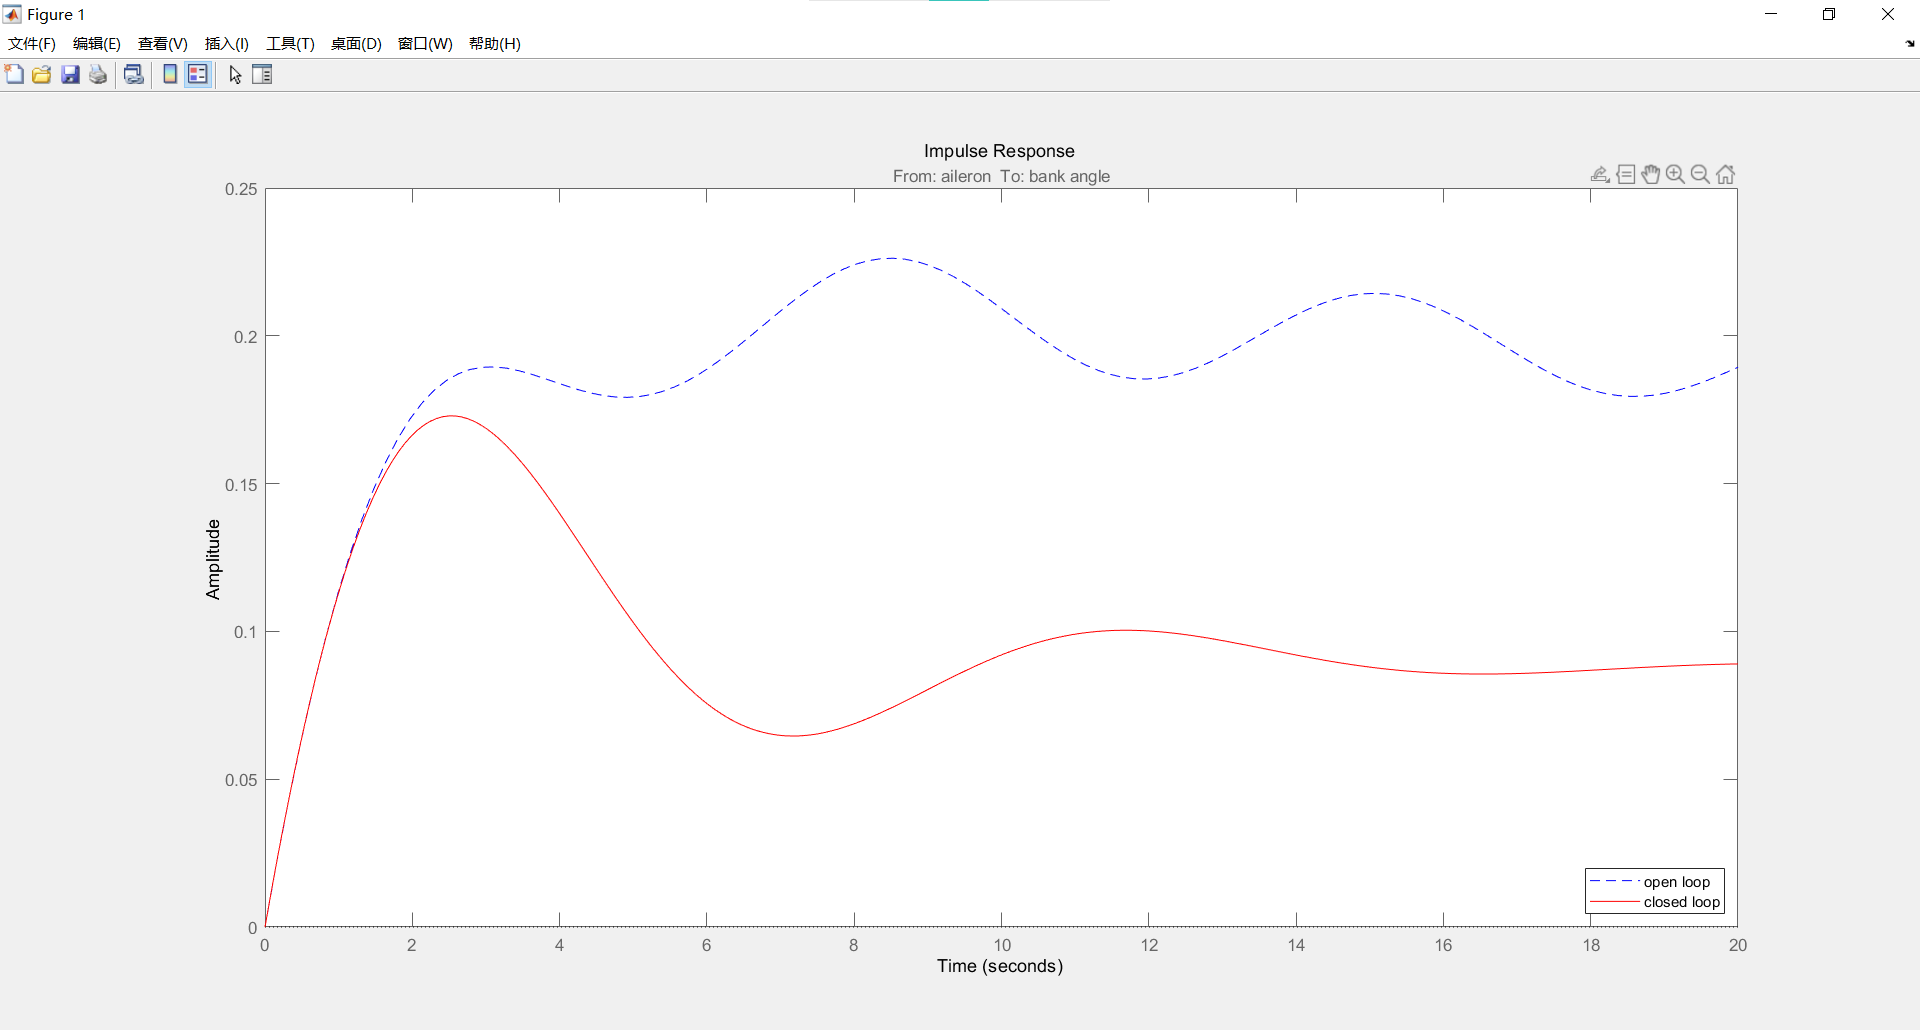
\includegraphics[width=350pt]{6.png}
    \caption{G. 分配中断号}
\end{figure}

H. 指定 NIos II 的复位和异常地址,从 ”System Contents” 标签栏双击建立好的 cpu 进入 Nios II Processor 的配置界面,配置 Reset Vector 和 Exception Vector 为下图中所示,点击 Finish。

I. 点击 Qsys 主界面菜单栏中的 ”System” 下的 ”Create Global Reset Network”。完成后会自动连接所有复位端口。

J. 生成 Qsys 系统,点选 ”Generation HDL” 标签栏中 Generate 按钮生成 Qsys 系统。

\begin{figure}[htbp]
    \centering
    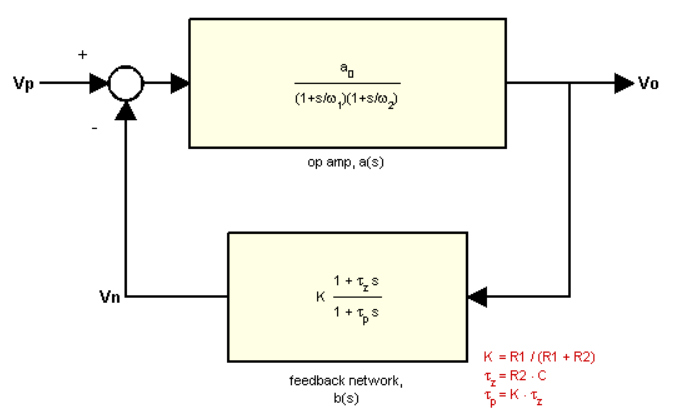
\includegraphics[width=350pt]{7.png}
    \caption{J. 生成 Qsys 系统}
\end{figure}

\section{其它模块的设计}
A. 时钟分频器

在该模块中,使用了两个寄存器 r 和 r1 来计数时钟周期。寄存器 r 是一个 25 位的计数器,用于计算时钟信号的周期。寄存器 r1 是一个 1 位的寄存器,用于控制时钟分频。使用 always \@(posedge clk or negedge n\_rst) 声明了两个时序块。这些时序块在时钟上升沿和异步复位边缘触发时执行。在第一个时序块中,当异步复位信号 n\_rst 为低电平时,计数器 r 被清零。否则,在时钟上升沿时,计数器 r 递增。当计数器 r 达到 25 位的最大值 24\_999\_999 时,计数器被重新设置为零。在第二个时序块中,当异步复位信号 n\_rst 为低电平时,寄存器 r1 被清零。否则,在时钟上升沿时,如果计数器 r 达到 25 位的最大值 24\_999\_999,则寄存器 r1 取反。最后,使用 assign 语句将 r1 寄存器的值赋给输出端口 tm\_scd。

module div25m(clk, n\_rst, tm\_scd);

input clk, n\_rst;

output tm\_scd;

reg [24:0]r;

always @(posedge clk or negedge n\_rst)

begin

	if(~n\_rst)

		r<=25'd0;

	else

	begin

		if(r==25'd24\_999\_999)

			r <=25'd0;

		else

			r <= r + 1'b1;

	end	

end

reg r1;

always @(posedge clk or negedge n\_rst)

begin

	if(~n\_rst)

		r1<=1'd0;

	else

	begin

		if(r==25'd24\_999\_999)

			r1 <= ~r1;

		else

			r1 <= r1;

	end	

end

assign tm\_scd = r1;

Endmodule

B. 锁存器模块
\begin{figure}[htbp]
    \centering
    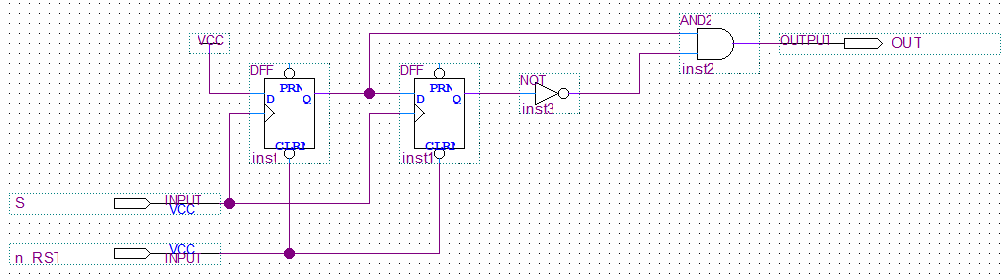
\includegraphics[width=350pt]{8.png}
    \caption{B. 锁存器模块}
\end{figure}

C. 频率选择器
该模块实现了一个频率选择器(Frequency Selector),根据选择信号 sel 的值来选择不同的输入信号 pa 或 pb 输出到 pout。使用了一个三目运算符 ?: 来根据选择信号 sel 的值选择要输出的信号。如果 sel 为真,则输出 pa,否则输出 pb。使用 assign 语句将选择的输入信号赋给输出端口 pout。

module frq\_sel(pa, pb, sel, pout);

input [23:0]pa, pb;

input sel;

output [23:0]pout;

assign pout = (sel) ?  pa :pb;

Endmodule

\section{整体模块设计}
整个频率计的工作流程如下:

A. 输入信号经过Latch模块进行捕获,触发有效信号。

B. 有效信号触发FRQ\_SEL模块,选择相应的计时器模块开始计时。

C. 选择的计时器模块开始计时,测量输入信号的持续时间。

D. 当计时器模块完成计时后,将结果保存到适当的寄存器中。

E. FRQ\_SEL模块再次接收有效信号,根据有效信号的状态选择另一个计时器模块。

F. 重复步骤C至步骤E,以测量另一状态(高电平或低电平)的持续时间。
\begin{figure}[htbp]
    \centering
    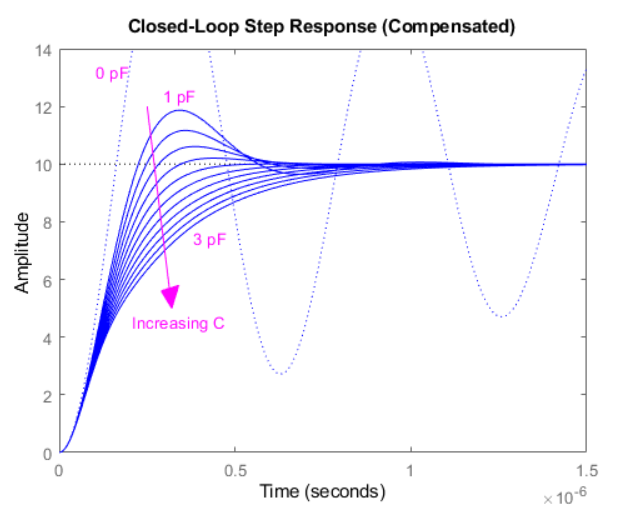
\includegraphics[width=350pt]{9.png}
    \caption{整体模块设计}
\end{figure}

\section{软件部分设计}
A. 启动 Nios II SBT,点击 Nios II Software Build Tools for Eclipse 打开 Nios II SBT for Eclipse
创建工程。

B. 在”SOPC Information File name”窗口中选择 kernel.sopcinfo文件,将生成硬件配置信息和软件应用关联。

C. 编写软件程序——C代码

\#include <stdio.h>

\#include <unistd.h>

\#include <altera\_avalon\_pio\_regs.h>

\#include <sys/alt\_irq.h>

volatile int counter = 0;

// 中断处理函数,在计数器每次溢出时触发

void isr(void* context)

{

    counter++;  // 每次溢出计数器加1

}

int main()

{

    alt\_ic\_isr\_register(TIMER\_IRQ\_INTERRUPT\_CONTROLLER\_ID, TIMER\_IRQ, isr, NULL, 0);  

    // 初始化计数器

IOWR\_ALTERA\_AVALON\_TIMER\_CONTROL(TIMER\_BASE, 0x07); // 启用计数器

IOWR\_ALTERA\_AVALON\_TIMER\_PERIODL(TIMER\_BASE, 0xFFFF);  // 设置计数器最大值

    // 等待一段时间让计数器计数

    usleep(1000000);
    
    // 停止计数器并禁用中断

    IOWR\_ALTERA\_AVALON\_TIMER\_CONTROL(TIMER\_BASE, 0x00);

    // 计算频率

    float frequency = (float)counter / 1000000; 

    printf("频率: %.2f Hz\n", frequency);

    return 0;

}

\chapter{实验设计总结及反思}
本次项目成功构建了一个Nios ii系统,并在野火的EP4CE10F17C8开发板实现了流水灯、数码管等简单例程。由于时间限制以及前期使用DE2-70开发板耽误较多时间,后面频率计只能自行课下设计,未能有机会上板测试验证。

这次暑期学校,通过使用Quartus II和SOPC Builder(Qsys),我学到了如何进行基于FPGA的硬件设计和开发,也了解了如何选择和配置外设、设置处理器参数以及创建系统连接,这为进一步深入研究和开发FPGA项目打下了基础。这个项目为我提供了一个综合性的学习机会,涵盖了硬件设计、嵌入式软件开发以及调试技巧等方面。通过实践和解决问题,积累了宝贵的经验,并提高自己在FPGA和嵌入式系统开发方面的能力。
\varsigma 
\backmatter


% %=======%
% %引入参考文献文件
% %=======%
\bibdatabase{bib/POC}%bib文件名称 仅修改bib/ 后部分
\printbib
\nocite{*} %显示数据库中有的,但是正文没有引用的文献


% \Appendix

% 这里是附录页,可要可不要

% \Thanks.



\end{document}